The definition of UCM metamodel and the specification of weaving algorithm described in the previous chapter provide the foundation for the implementation of UCM in TouchCORE, a multitouch-enabled concern-oriented software design modeling tool. In this chapter, we illustrate the realization of scenario models in TouchCORE through the use of UCM notation in section~\ref{sec:4.1}. Then we attempt to validate our proposed approach of concern-oriented UCMs by means of case studies in section~\ref{sec:4.2}. Finally, we demonstrate that concern-oriented UCMs are able to cover the workflow patterns in section~\ref{sec:4.3}.

\section{UCM Implementation in TouchCORE} \label{sec:4.1}

TouchCORE is under active development within the Software Engineering Lab at McGill University \cite{sel2015touchcore}. Previous project, TouchRAM, successfully implemented concern-oriented software design paradigm, but support is limited to RAM (class, sequence, and state diagrams) \cite{al2012touchram, schottle2014touchram}. TouchCORE extends TouchRAM with numerous enhancements, and most notably, the support for arbitrary modeling languages in addition to RAM. Since we have a well-defined corified UCM metamodel, we attempted to add support for UCMs in TouchCORE as proof of concept, enabling TouchCORE the capability to build scalable and reusable scenario models.

The project uses Java SE Development Kit 8 as the implementation language and Eclipse Modeling Framework (EMF)~\cite{steinberg2008emf} as the modeling facility for developing TouchCORE. To support a new language, we need to define its metamodel based on Ecore. TouchCORE already has a complete CORE metamodel defined with an Ecore model (see Figure~\ref{fig:a.1}). With RAM as a reference model, we constructed an Ecore model that expresses our complete UCM metamodel, subclassing the appropriate CORE metaclasses, through the use of EMF tooling (see Figure~\ref{fig:a.2}). EMF is capable of generating structured Java code from valid Ecore models, allowing us to rapidly program the logic for UCM integration.

\begin{figure}
	\centering
	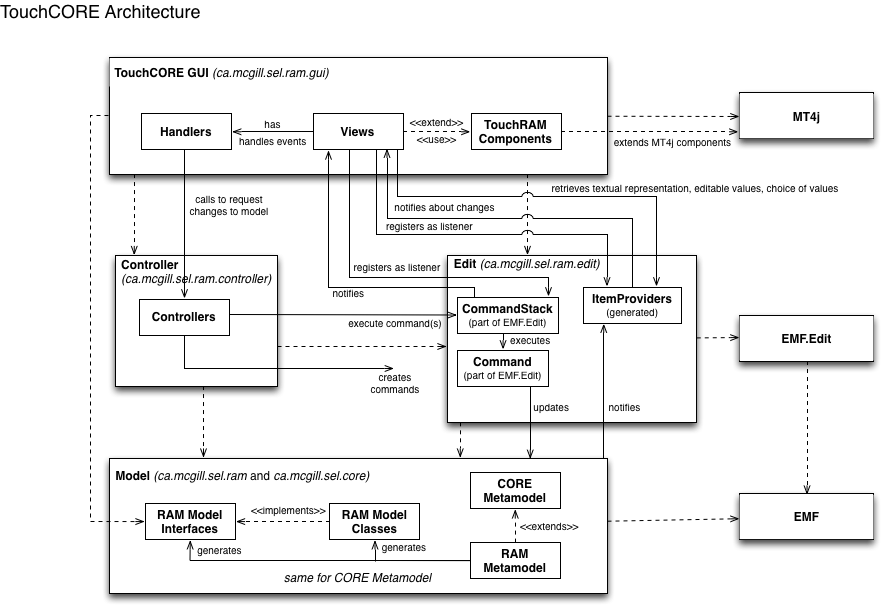
\includegraphics[scale=0.5]{fig_4_1.png}
	\caption[TouchCORE architecture]{TouchCORE architecture. Image courtesy of Software Engineering Lab, McGill University}
	\label{fig:4.1}
\end{figure}

The software architecture of TouchCORE follows the model–view–controller (MVC) design pattern to separate the program into three main logical components. Figure~\ref{fig:4.1} shows the three interconnected parts for the TouchCORE application: (i) the model layer for managing data, e.g., instances of RAM and UCM models; (ii) the TouchCORE graphical user interface (GUI) that constitutes the view layer for visualizing and manipulating models; and (iii) the controller layer for handling user interactions and act on the data model objects. The GUI for TouchCORE is built on top of MT4j for its multitouch capability \cite{laufs2010mt4j}. Additional components include weaver, code generator, model validator, and classloader. The integration of UCM in TouchCORE involves modifying its core components with varying degrees, but the program is structured in such a way that we can add subcomponents when implementing a new modeling language, adhering to the open/closed principle.

\subsection{Supported Concrete Syntax}

\begin{figure}[h]
	\centering
	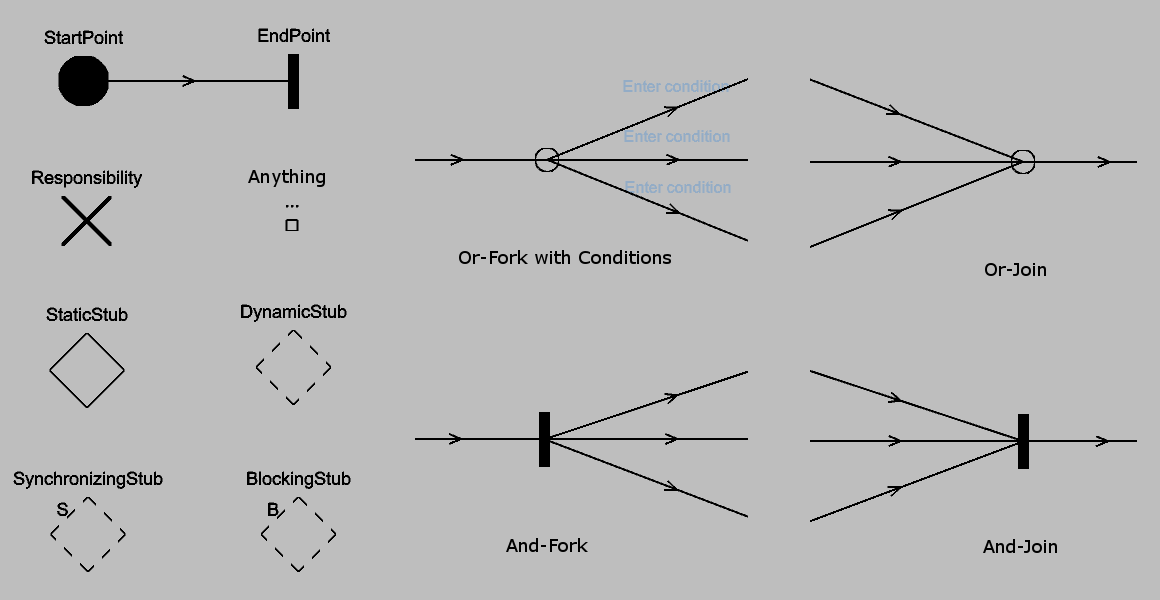
\includegraphics[scale=0.3]{fig_4_2.png}
	\caption{UCM notation in TouchCORE}
	\label{fig:4.2}
\end{figure}

The basic elements of the UCM notation that we implemented in TouchCORE are shown in Figure~\ref{fig:4.2}. Most of these elements are defined by the standards~\cite{itu2012151}, with the exception of {\cls Anything} that is taken from the extended AoUCM metamodel~\cite{mussbacher2011aspect}. Users can create path nodes by tap-and-hold on the canvas of TouchCORE during runtime and a list of path node selection will be displayed. To create a node connection between two path nodes, simply drag from the area adjacent of one element to the other element.

There are several anomalies with regards to the graphical representation of UCM symbols displayed in TouchCORE as compared with the standards (compare Figure~\ref{fig:4.2} with Figure~\ref{fig:2.7}). For example, the symbol for or-fork and or-join is shown as a circle instead of no symbol (just direct branching and merging from the paths); anything is represented as a square with the label \ldots\ instead of just \ldots; and node connection is a straight line path instead of spline. These are some of the limitations that we faced at the moment when implementing the GUI. Our current method of creating nodes is to first create them on the canvas, then build the connections later. Or-fork and or-join need a space to receive events from the user, thus a circle serves as the area of interactivity as well as a statement of presence that an or-fork or or-join has been created. The idea of displaying the \ldots symbol of an anything node is that it should be part of the node connection and move along seamlessly with correct orientation whenever the predecessor or successor node of anything is moved, but since anything is considered a path node, we decided for now to just use a square with the label \ldots\ to represent the anything node. Lastly, spline drawing is not yet available in TouchCORE so we use straight lines for the time being.

\begin{figure}
	\centering
	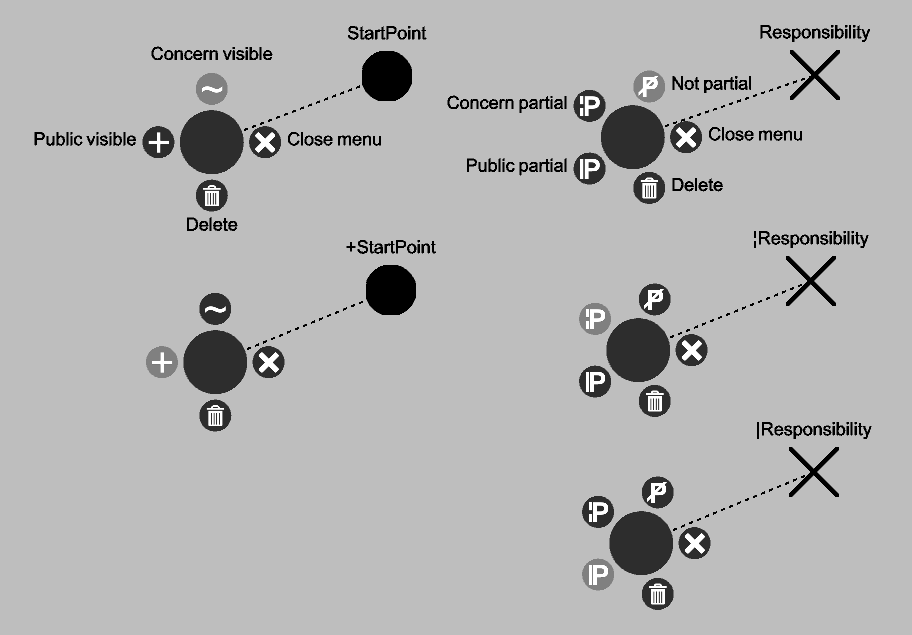
\includegraphics[scale=0.3]{fig_4_3.png}
	\caption{Visibility and partiality}
	\label{fig:4.3}
\end{figure}

Elements with extra features can be accessed by tap-and-hold an element (Figure~\ref{fig:4.3}). We allow start and end points to set its visibility. By default, all path nodes are concern visible, but start and end points can switch to public visible (see Section~\ref{sec:3.2.1.1} for visibility discussion). Likewise, we allow responsibilities to set its partiality. By default, all path nodes are not partial, meaning that they are well-defined and require no further action. Since we have customization mappings for responsibility, we can specify whether a responsibility is partially defined and require appropriate composition to be semantically complete. A responsibility that is concern partial should fulfill its significance through model extension, whereas a responsibility that is public partial should fulfill its significance through model reuse.

\subsection{Scenario Model Composition}

\subsubsection{Model Extension}

\subsubsection{Model Reuse}

\section{Case Studies} \label{sec:4.2}

\subsection{Authentication}

%\cite{amyot2012concern, thimmegowda2014concern}

\subsection{Online Payment}

%\cite{w3c2015web}

\section{Workflow Patterns} \label{sec:4.3}

%\cite{van2003workflow}
%\cite{mussbacher2007evolving}
